\section{Distributed Model Checking} \label{sec::DMC}
In addition to benefiting from the isolation of actors for reducing the size of state spaces, this property can be used for more efficient analysis of huge state spaces. A major limiting factor in applying model checking for the analysis of real-world systems is the huge amount of memory space and time required to store and explore state spaces. Distributed model checking is a technique for analyzing the state space in which it is partitioned into slices and each slice is assigned to a computational node to be analyzed. Efficiency of this technique depends on the number of required communications among the computational nodes which is affected by the distribution policy of states among the nodes \cite{DBLP:journals/entcs/OrzanPE05}. 
%
%Another, more fine-grained, representative of communication cost 
To reduce the number of required communications, split transitions have to be avoided; a split transition is a transition between two states where the hosts of the source and destination states are located at different nodes. In \cite{DBLP:journals/eceasst/KhamespanahSMSR15} we show how the actor model can be used to reduce the number of split transitions. We introduce a new state distribution policy based on the so-called \textit{Call Dependency Graph (CDG)} of actor models. A CDG represents the abstract causality relation among messages of actors. Our abstraction is akin to the Clinger's event diagram \cite{clinger} that shows the causality among events which are sent by actors of the system in their life times. Note that sent messages in CDG are interpreted as events in the Clinger's event diagram.

The most primitive and widely used distribution policy is random state distribution \cite{DBLP:journals/entcs/GaravelMS13}. Random state distribution policy distributes states among nodes based on their hash values. Random distribution policy guarantees load balancing. However, it is not an effective technique as cycles in the state space are scattered over many different nodes. Note that detecting cycles of state spaces is crucial for model checking against LTL-like properties; so, splitting them among nodes (i.e., reducing locality of cycles) dramatically increases the model checking time consumption. In \cite{DBLP:journals/entcs/OrzanPE05}, another state space distribution policy is suggested to improve the locality of cycles. This policy is based on the static analysis of an abstracted model and detects \emph{may} or \emph{must} transition relations among states \cite{DBLP:conf/lics/LarsenT88}.
\fixme{define may and must in one sentence}
Based on this analysis, if two states have a \emph{must} relation, they should be stored in a same node. We use a similar idea in our state distribution policy using CDG by partitioning causality relations of CDGs to \emph{may} and \emph{must} relations. So, we detect the \emph{must} relations among the states of an actor model considering the cycles of its corresponding CDG and putting them in the same node. Our technique is applicable to other distributed systems where the unit of concurrency can be modeled as isolated autonomous reactive objects and message passing is the only means of communication. 

Clinger's event diagram comprises vertices (called \emph{dots}) for each event, and edges (called \emph{arrows}) that represent the activation relation of two events. Clinger's event diagram is typically drawn using parallel vertical swim-lanes for each actor, where the dots are placed for each event respecting their sequential execution order. Figure~\ref{fig::clinger} represents the Clingers' event diagram of a simple actor model, shown in Listing~\ref{src::actor-model}. 

\begin{lstlisting}[language=rebeca, caption= A simple actor model, label=src::actor-model]
reactiveclass AC1 {
   knownrebecs {AC2 ac2;}
   AC1() {
     self.msg1();
   }
   msgsrv msg1() {
     self.msg2();
     ac2.msg3();
   }
   msgsrv msg2() {
     self.msg1();
     ac2.msg4();
   }
}
reactiveclass AC2 {
   knownrebecs{AC1 ac1;}
   statevars{int sv;}
   AC2() {
     sv = 1;
   }
   msgsrv msg3() {
     ac1.msg1();
   }
   msgsrv msg4() {
     if (sv == 1)
       sv = 4;
     else
       sv = 3;
   }
}
main {
    AC1 ac1(ac2):();
    AC2 ac2(ac1):();
}
\end{lstlisting}

Clinger's event diagrams can be seen as the detailed representations of CDG. As actors are isolated, the only causality relation among events is expressed by sending a message. So, the causality relation of events in a CDG can be extracted from the source codes of actor models using static analysis. This way, we over-approximate the causality relations in CDGs. Figure \ref{fig::cdg} illustrates the CDG which corresponds to the Clinger's event diagram of Figure \ref{fig::clinger}.

\begin{figure}
\centering
%\subfigure[Clinger event diagram of the actor model in Listing \ref{src::actor-model}]{
\begin{subfigure}[b]{0.2\textwidth}
  \centering
  \small{
   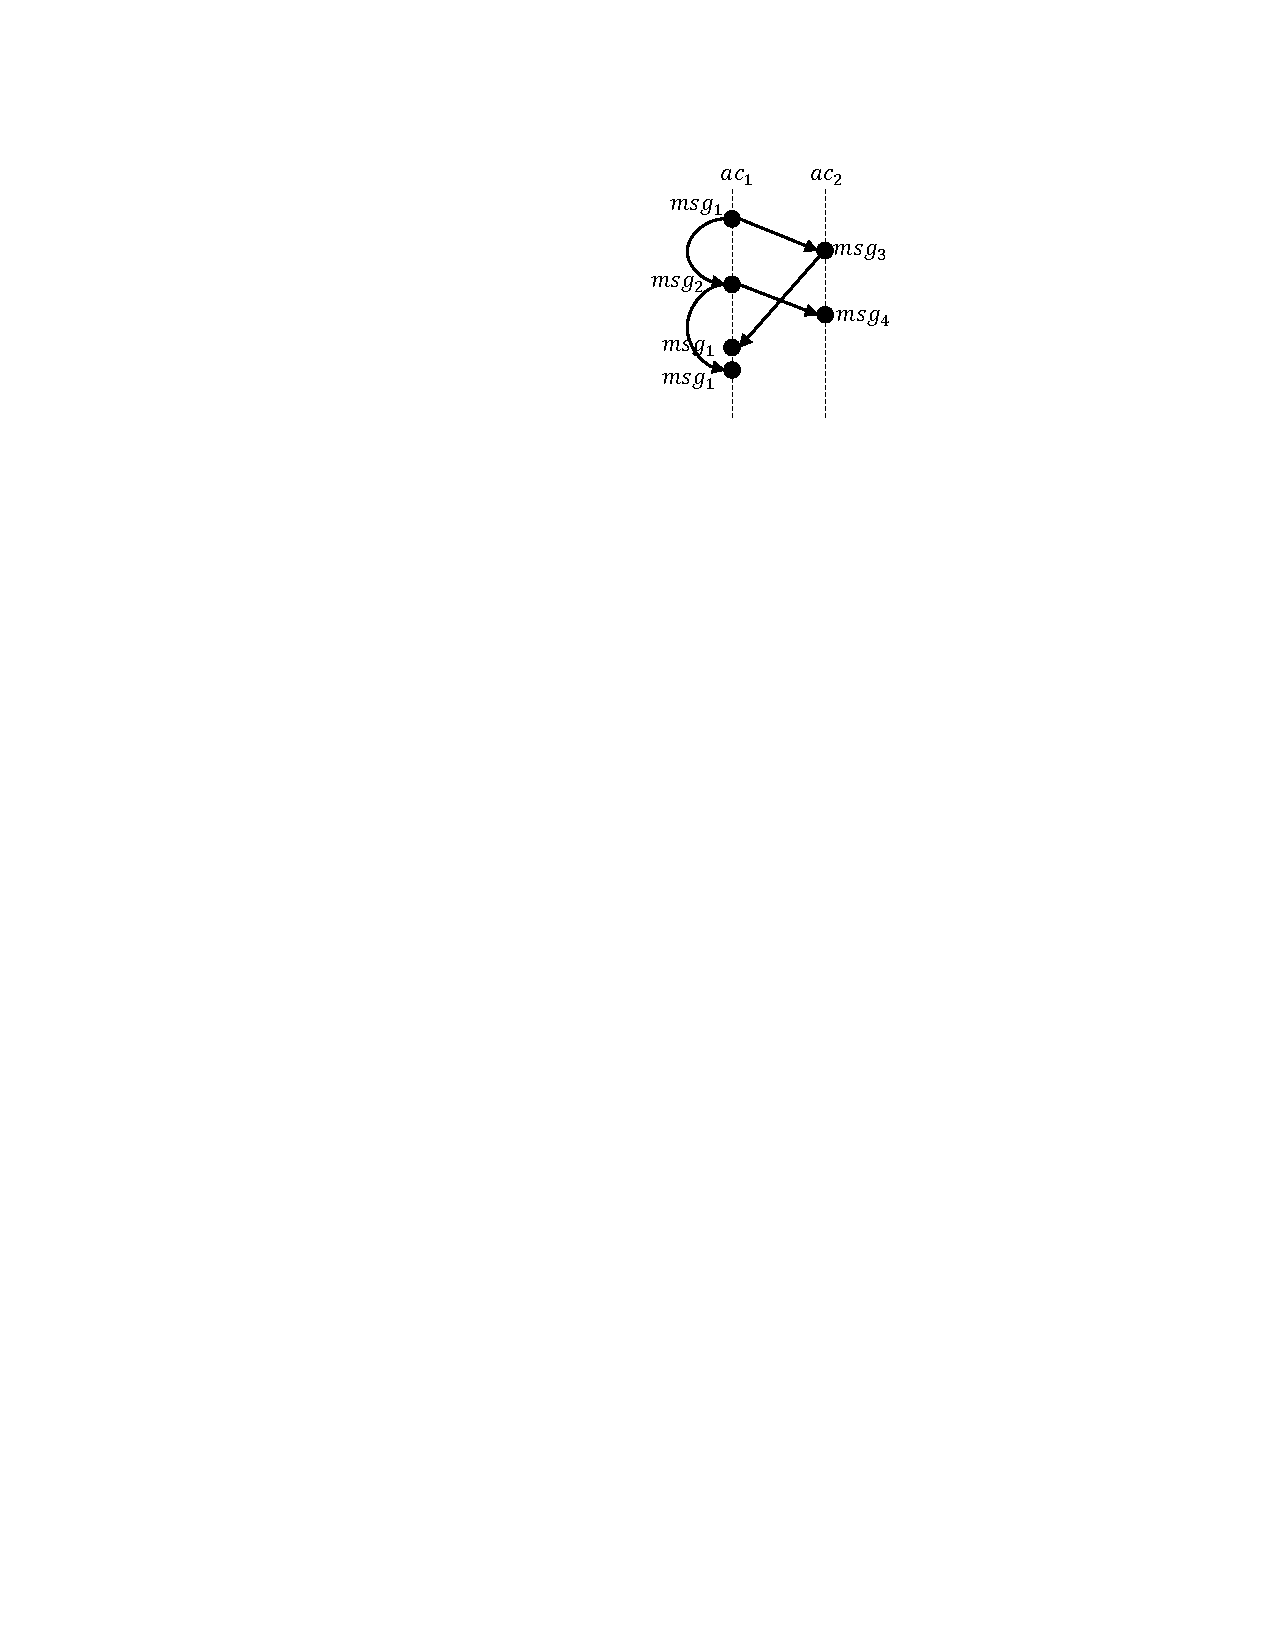
\includegraphics[width=.8\textwidth]{resources/clinger.pdf}
  }
  \caption{Clinger event diagram of the actor model in Listing \ref{src::actor-model}}
  \label{fig::clinger}
%}
\end{subfigure}
\qquad
\begin{subfigure}[b]{0.2\textwidth}
%\subfigure[CDG of the actor model in Listing 1]{

  \centering
  \small{
   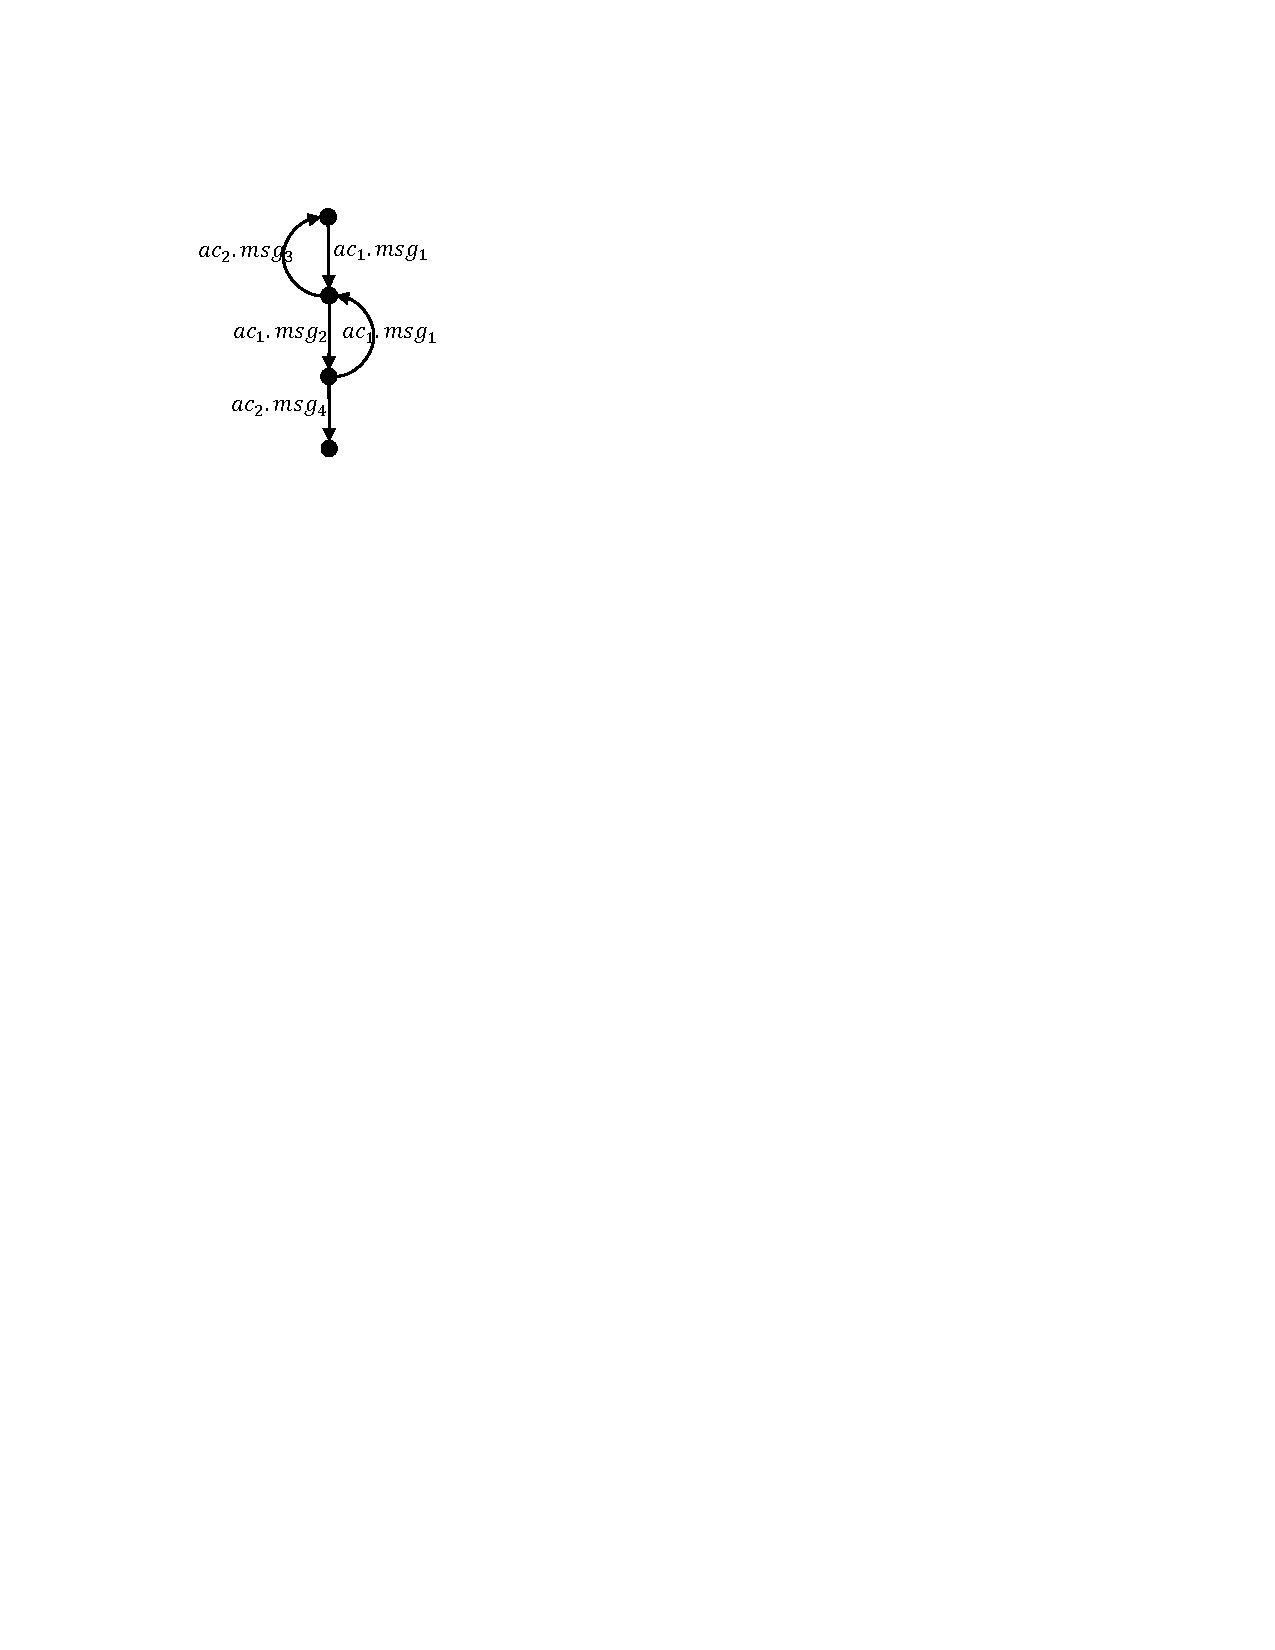
\includegraphics[width=.8\textwidth]{resources/cdg.pdf}
  }
  \caption{CDG of the actor model in Listing \ref{src::actor-model}}
  \label{fig::cdg}
%}
\end{subfigure}
\caption{Clinger event diagram versus CDG of the actor model in Listing \ref{src::actor-model}.}
\label{fig::clinger-cdg}
\end{figure}

We designated the existence of a relation between the cycles in a CDG and the cycles in its corresponding state space in \cite{DBLP:journals/eceasst/KhamespanahSMSR15}. \Fatem{It is not clear that how isolation helps in resolving this issue}. 
As mentioned before, Rebeca actors are completely isolated and the only way of expressing causality among events is the message passing mechanism, explicitly specified in Rebeca models. Experimental evidence supports that this new policy improves cycles locality, and decreases the model checking time and memory consumption in practice.